\documentclass[../../main.tex]{subfiles}

\graphicspath{{../../image/}{../../figure/}}

\begin{document}

\section{概率图模型}\label{section:ch11-概率图模型}

我们已经看到，概率是深度学习最重要的基础概念之一。例如，用于二元分类的神经网络可以用一个条件概率分布来描述，其形式为

\begin{align}
  p(t\mid \mathbf{x},\mathbf{w}) = y(\mathbf{x},\mathbf{w})^{\,t}\,\bigl(1-y(\mathbf{x},\mathbf{w})\bigr)^{\,1-t}
  \label{align:ch11-二元分类条件分布}
\end{align}

其中，$y(\mathbf{x},\mathbf{w})$表示神经网络函数，它以向量$\mathbf{x}$作为输入，并受可学习参数向量$\mathbf{w}$的控制。相应的交叉熵似然是构建用于训练神经网络的误差函数的基础。虽然神经网络函数可能极其复杂，但式~\eqref{align:ch11-二元分类条件分布}中的条件分布形式却很简单。有许多重要的深度学习模型都具有更丰富的概率结构，如大语言模型、归一化流、变分自编码器、扩散模型等。为了描述和利用这种结构，我们引入了一个强大的框架，称为概率图模型（probabilistic graphical model）或简称图模型（graphical model），它允许以图的形式表达结构化概率分布。当与神经网络相结合来定义相关的概率分布时，图模型为创建可以端到端训练的复杂模型提供了巨大的灵活性，其中梯度可通过自动微分来进行有效计算，并使用随机梯度下降进行训练。本章将重点讨论应用深度学习所需的概率图模型的核心概念，而对机器学习的概率图模型更为全面的讨论可参阅 Bishop (2006)。

概率可以用两个简单的法则来表示，即加和法则和乘积法则（参见2.1节）。本书讨论的所有概率操作，无论多么复杂，都相当于重复应用这两个法则。因此，原则上我们可以纯粹通过代数操作来制定和使用复杂的概率模型。不过，我们发现使用概率分布的图示法来扩充分析是有好处的，因为图示法具有以下3个有用的特性：

\begin{enumerate}
  \item 它们提供了一种可视化概率模型结构的简单方法，可用于设计和构思新的模型；
  \item 通过对图进行检查，可以深入了解模型的特性，包括条件独立性；
  \item 在复杂模型中进行推理和学习所需的复杂计算可以用图形操作来表示，如消除消息传递，其中隐式地进行了基本的数学运算。
\end{enumerate}

\subsection{有向图}\label{subsection:ch11-有向图}

图由节点（也称顶点）构成，这些节点由边来连接。在图模型中，每个节点代表一个随机变量，而连接则表示这些变量之间的概率关系。然后，图就可以记录所有随机变量的联合分布是如何分解成多个因子（每个因子都仅依赖变量的一个子集）的乘积的。本章将重点讨论图模型，在图模型中，图的连接具有箭头指示的特定方向。这些模型称为有向图模型（directed graphical model），也称贝叶斯网络。有向图适用于表达随机变量之间的因果关系，而无向图更适合表达随机变量之间的软约束。图模型的另一大类是马尔可夫随机场（Markov random field），也称无向图模型（undirected graphical model），其中的连接不带箭头，无方向意义。有向图和无向图都可以看作一种叫作因子图（factor graph）表示法的特例。接下来，我们将重点关注有向图。不过，请注意，在我们讨论图神经网络（Graph Neural Network, GNN）（参见第13章）时（其中节点代表标准神经网络中的确定性变量），也会出现无概率解释的无向图。

虽然这种概率图模型的节点和边与神经网络图很相似，但它们具有特别的概率性解释，并含有更丰富的语义。为了避免混淆，本书用蓝色表示神经网络图，用红色表示概率图模型（后文简称图模型）。

\subsection{分解}\label{subsection:ch11-分解}

为了有利于使用有向图描述概率分布，首先考虑关于3个变量$a$、$b$和$c$的任意联合分布$p(a,b,c)$。请注意，在这个阶段，我们不需要进一步说明它们都是些什么变量，比如它们是离散变量还是连续变量。事实上，图模型的一个强大之处在于，一个特定的图可以为多个分布类别做出概率说明。通过应用概率的乘积法则（式(2.9)），我们可以写下联合分布，形式如下：

\begin{align}
  p(a,b,c) = p(c\mid a,b)\,p(a,b)
  \label{align:ch11-三变量分解1}
\end{align}

再次应用乘积法则对式~\eqref{align:ch11-三变量分解1}右边的第二项进行计算，得到

\begin{align}
  p(a,b,c) = p(c\mid a,b)\,p(b\mid a)\,p(a)
  \label{align:ch11-三变量分解2}
\end{align}

请注意，无论选择何种联合分布，以上分解都是成立的。下面让我们用一个简单的图模型来表示式~\eqref{align:ch11-三变量分解2}的右侧，如图11.1所示。首先为随机变量$a$、$b$和$c$分别引入一个节点，并将每个节点与式~\eqref{align:ch11-三变量分解2}右侧相应的条件分布联系起来。然后为每个条件分布添加有向连接（如箭头所示），这些连接来自与分布条件变量相对应的节点。因此，对于因子$p(c\mid a,b)$，将存在从节点$a$和$b$到节点$c$的连接；而对于因子$p(a)$，则不存在传入连接。如果节点$a$和节点$b$之间存在一个连接，那么节点$a$是节点$b$的父节点，相应地，节点$b$是节点$a$的子节点。请注意，我们不会对节点以及节点所对应的变量进行任何形式上的区分，而只是使用相同的符号指代两者。

\begin{figure}[htbp]
  \centering
  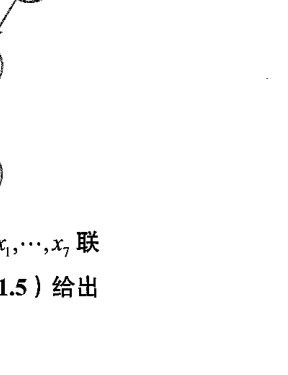
\includegraphics[width=0.55\textwidth]{ch11-fig311-directed-graph.png}
  \caption{一个描述变量$x_1,\cdots,x_7$联合分布的有向图，对应于式~\eqref{align:ch11-7变量分解}的分解。}
  \label{figure:ch11-有向图分解}
\end{figure}

对于式~\eqref{align:ch11-三变量分解2}，重要的一点是，它的左侧变量与变量$a$、$b$、$c$是对称的，而右侧变量则不对称。在对式~\eqref{align:ch11-三变量分解2}进行分解时，我们隐式地选择了一种特定的排序，即$a$、$b$、$c$；如果我们选择不同的排序，就会得到不同的分解，从而得到不同的图形化表示。

下面让我们通过$p(x_1,\cdots,x_K)$给出的$K$个变量的联合分布来扩展图11.1中的示例。通过反复应用乘积法则，该联合分布可以写成条件分布的乘积，$K$个变量中的每一个变量都有一个条件分布：

\begin{align}
  p(x_1,\cdots,x_K) = p(x_K\mid x_1,\cdots,x_{K-1})\cdots p(x_2\mid x_1)\,p(x_1)
  \label{align:ch11-K变量分解}
\end{align}

对于给定的$K$，我们可以再次将这表示为一个有向图，其中有$K$个节点。式~\eqref{align:ch11-K变量分解}右侧的每个条件分布都有一个节点，且每个节点都有来自所有较低编号节点的输入连接。我们称这个图是全连接的（fully connected），因为每一对节点之间都有一个连接。

到目前为止，我们使用的都是完全通用的联合分布，因此它们的分解和相关的全连接图表示适用于任何分布。我们很快就会发现，正是图中没有（absence）的连接传达了关于图所代表的分布类属性的有趣信息。参见图11.2所示的有向图。请注意，这并不是一个全连接图，因为从节点$x_1$到$x_3$或者从节点$x_3$到$x_4$并不存在连接。从这个有向图中提取出联合（概率）分布的相应表示，即图11.2给出了联合分布的相应分解。例如，节点$x_6$将以节点$x_2$和$x_4$为条件。因此，所有7个变量的联合分布为

\begin{align}
  p(x_1,\cdots,x_7) = p(x_1)\,p(x_2)\,p(x_3)\,p(x_4\mid x_1,x_2,x_3)\,p(x_5\mid x_1)\,p(x_6\mid x_4)\,p(x_7\mid x_4,x_5)
  \label{align:ch11-7变量分解}
\end{align}

我们现在所讨论的有向图有一个重要的限制条件，即禁止存在有向环（directed cycle）。换句话说，图中不存在闭环路径，这意味着我们不能沿着箭头的方向从一个节点移动到另一个节点，最后回到起始节点。这种图也称有向无环图，或简称DAG（Directed Acyclic Graph）。这表示存在一种节点排序，使得不存在从任何节点到任何较低编号节点的连接（见习题11.2）。

现在，我们可以用一般性术语来说明给定有向图与相应变量分布之间的关系。图定义的联合分布由图中所有节点的条件分布的乘积给出，每个节点的条件分布以图中该节点的父节点所对应的变量为条件。因此，对于一个有$K$个节点的图，联合分布的计算公式为

\begin{align}
  p(\mathbf{x}) = \prod_{k=1}^{K} p\bigl(x_k\mid \mathrm{pa}(x_k)\bigr)
  \label{align:ch11-有向图联合分布}
\end{align}

其中，$p\bigl(\mathrm{pa}(x_k)\bigr)$表示节点$x_k$的父节点集。这个关键公式表达了有向图模型联合分布的分解特性。虽然每个节点对应一个变量，但我们同样可以将变量集、向量值变量或张量值变量与图中的节点联系起来。不难看出，只要各个条件分布被归一化，式~\eqref{align:ch11-有向图联合分布}右侧的表示就总是能被正确地归一化（见习题11.1）。建议读者花点时间仔细研究一下式~\eqref{align:ch11-7变量分解}与图11.2之间的对应关系。

\subsection{离散变量}\label{subsection:ch11-离散变量}

我们已经讨论过作为指数族分布成员的概率分布的重要性，并看到指数族分布中包括许多知名分布的特例（参见3.4节）。虽然这些分布相对简单，但它们构成了构建更复杂概率分布的有用构件，而图模型非常有助于表达这些构件是如何相互连接在一起的。对于广泛使用的组件分布，有两种特殊的选择，分别对应于离散变量和高斯变量。我们先来看看离散变量。

具有$K$种可能状态（使用1-of-$K$表示法）的单个离散变量$x$的概率分布$p(x\mid \boldsymbol{\mu})$由下式给出并由参数$\boldsymbol{\mu}=(\mu_1,\cdots,\mu_K)$控制：

\begin{align}
  p(x\mid \boldsymbol{\mu}) = \prod_{k=1}^{K}\mu_k^{x_k}
  \label{align:ch11-离散变量分布}
\end{align}

由于约束$\sum_k \mu_k = 1$，因此只需要指定$\boldsymbol{\mu}$的$K-1$个值即可定义分布。假设有两个离散变量$x_1$和$x_2$，其中每个变量都有$K$种状态，希望模拟它们的联合分布。用参数$\mu_{ij}$表示同时观测到$x_1=i$和$x_2=j$的概率，其中$x_{1i}$表示$x_1$的第$i$个组件，$x_{2j}$表示$x_2$的第$j$个组件。联合分布可以写为$p(x_1,x_2\mid \boldsymbol{\mu})=\prod_{i,j}\mu_{ij}^{x_{1i}x_{2j}}$。由于参数$\mu_{ij}$受$\sum_{i,j}\mu_{ij}=1$的约束，因此以上联合分布受$K^2-1$个参数的控制。

利用乘积法则，我们可以将联合分布$p(x_1,x_2)$分解为$p(x_2\mid x_1)\,p(x_1)$的形式，对应于一个两节点图，其中有一个从节点$x_1$到节点$x_2$的连接，如图11.3(a)所示。边缘分布$p(x_1)$和之前一样受$K-1$个参数的控制。同样，条件分布$p(x_2\mid x_1)$需要为$x_2$的$K$个可能取值中的每个值指定$K-1$个参数。因此，在联合分布中必须指定的参数总数依然是$(K-1)+K(K-1)=K^2-1$。

假设变量$x_1$和$x_2$是独立的，对应于图11.3(b)所示的图模型。然后，将每个变量都用一个独立的离散分布来描述，参数总数为$2(K-1)$。对于$M$个独立离散变量的分布（每个变量有$K$个状态），参数总数为$M(K-1)$，因此参数总数随着变量数量的增加而呈线性增长。从图的角度来看，我们已经通过放弃图中的连接来减少参数的数量，但这样做的代价是分布的类更加有限了。

更一般地说，如果有$M$个离散变量$x_1,\cdots,x_M$，则可以使用有向图对联合分布进行建模，每个节点有一个变量。每个节点上的条件分布由一组非负参数给出，这些参数受限于归一化约束。如果图是全连接的，那么我们就有了一个完全通用的分布，该分布有$K^M-1$个参数；而如果图中没有连接，联合分布就会分解为边缘分布的乘积，参数总数为$M(K-1)$。具有中间水平连通性的图比完全分解的图更易于实现一般分布，且比一般分布需要更少的参数。如图11.4所示，边缘分布$p(x_1)$需要$K-1$个参数，而对于$i=2,\cdots,M$，条件分布$p(x_i\mid x_{i-1})$中的每个分布都需要$K(K-1)$个参数。因此这个具有$M$个离散节点（每个节点有$K$个状态）的节点链需要指定$K-1+(M-1)K(K-1)$个参数，总的参数数量为$K-1+(M-1)K(K-1)$，与节点链长度$M$的增加呈线性增长（而非指数增长）。相比之下，由$M$个节点组成的全连接图则有$K^M-1$个参数，参数的数量随着$M$的增加量指数增长。

共享参数（也称捆绑参数）是减少模型中独立参数数量的另一种方法。例如，在图11.4中，我们可以安排在$i=2,\cdots,M$的情况下，所有条件分布$p(x_i\mid x_{i-1})$都受同一组$K(K-1)$个参数的控制，从而得到图11.5所示的模型。再加上控制$x_1$分布的$K-1$个参数，总共需要指定$K^2-1$个参数来定义联合分布。

在离散变量模型中，控制参数数量增长的另一种方法是使用参数化的条件分布表，而非使用完整的条件概率值表。为了阐明这一观点，请看图11.6所示的模型，其中所有节点都代表二进制变量。每个父变量$x_i$由代表概率$p(x_i=1)$的单个参数$\mu_i$控制，其中所有节点都代表二进制变量。每个父变量$x_i$由代表概率$p(x_i=1)$的单个参数$\mu_i$控制，因此父节点共有$M$个参数。然而，条件分布$p(y\mid x_1,\cdots,x_M)$需要$2^M$个参数，用于表示父变量$2^M$种可能设置中每一种设置的概率$p(y=1)$。因此，一般来说，指定这一条件分布所需的参数数量将随着$M$的增加呈指数增长。通过使用作用于父变量线性组合的逻辑斯谛sigmoid函数（参见3.4节），我们可以得到如下更简洁的条件分布形式：

\begin{align}
  p(y=1\mid x_0,x_1,\cdots,x_M) = \sigma\left(\sum_{i=0}^{M} w_i x_i\right) = \sigma\left(\mathbf{w}^{\mathsf{T}}\mathbf{x}\right)
  \label{align:ch11-逻辑斯谛条件分布}
\end{align}

其中，$\sigma(a)=(1+\exp(-a))^{-1}$是逻辑斯谛sigmoid函数，$\mathbf{x}=(x_0,x_1,\cdots,x_M)$是一个$(M+1)$维的父状态向量，其中增加了一个变量$x_0$，其值限制为1，而$\mathbf{w}=(w_0,w_1,\cdots,w_M)$是一个包含$M+1$个参数的向量。与一般情况相比，这种条件分布的形式更受限制，但它现在受一些随$M$的增加呈线性增长的参数的控制。从这个意义上讲，这类似于在多元高斯分布中选择协方差矩阵的限制形式（例如对角矩阵）。

\subsection{高斯变量}\label{subsection:ch11-高斯变量}

让我们回到图模型，其中节点代表具有高斯分布的连续变量。每个分布都以图中父节点的状态为条件。这种依赖关系可以有多种形式，这里我们重点讨论一种特定的选择，即每个高斯分布的均值是高斯父变量状态的某个线性函数。这就产生了另一类模型——线性高斯模型，其中包括许多具有实际意义的案例，如概率主成分分析（见16.2节）、因子分析和线性动态系统等（Roweis and Ghahramani, 1999）。

考虑$D$个变量上的任意一个有向无环图，其中节点$i$代表具有高斯分布的单个连续随机变量$x_i$。该高斯分布的均值是节点$i$的父节点$\mathrm{pa}(i)$状态的线性组合：

\begin{align}
  p\bigl(x_i\mid \mathrm{pa}(i)\bigr) = \mathcal{N}\left(x_i\,\Bigm|\, \sum_{j\in \mathrm{pa}(i)} w_{ij}x_j + b_i,\; v_i\right)
  \label{align:ch11-线性高斯条件}
\end{align}

其中$w_{ij}$和$b_i$是控制均值的参数，$v_i$是$x_i$条件分布的方差。联合分布的对数就是图中所有节点的这些条件式乘积的对数，因此其形式为

\begin{align}
  \ln p(\mathbf{x}) = -\frac{1}{2}\sum_{i=1}^{D}\frac{\left(x_i - \sum_{j} w_{ij}x_j - b_i\right)^2}{v_i} + \mathrm{const}
  \label{align:ch11-线性高斯对数}
\end{align}

其中$\mathbf{x}=(x_1,\cdots,x_D)$，且$\mathrm{const}$表示与$\mathbf{x}$无关的常数项。可以看到，这是$\mathbf{x}$的组件的二次函数，因此联合分布$p(\mathbf{x})$是多元高斯分布。

我们可以使用以下方法求出该联合分布的均值和协方差。每个变量的均值由递推公式给出（见习题11.6）：

\begin{align}
  \mathbb{E}[x_i] = \sum_{j} w_{ij}\,\mathbb{E}[x_j] + b_i
  \label{align:ch11-均值递推}
\end{align}

因此我们可以从最低编号的节点开始，通过图递归地找到$\mathbb{E}[\mathbf{x}]=(\mathbb{E}[x_1],\cdots,\mathbb{E}[x_D])$。同样，联合分布的协方差矩阵元素也满足以下形式的递推公式（见习题11.7）：

\begin{align}
  \mathrm{cov}[x_i,x_j] = \sum_{k} w_{ik}\,\mathrm{cov}[x_k,x_j] + \delta_{ij} v_i
  \label{align:ch11-协方差递推}
\end{align}

其中我们假设每个节点的编号大于其父节点的编号。因此，协方差同样可以从最低编号的节点开始递归求值。

考虑两个可能出现的图结构极端案例。首先，假设图中无连接，因此图由$D$个孤立节点构成。在这个情况下，参数$w_{ij}$不存在，因此只有$D$个参数$b_i$和$D$个参数$v_i$。从递推公式~\eqref{align:ch11-均值递推}和~\eqref{align:ch11-协方差递推}中可以看出，$p(\mathbf{x})$的均值为$(b_1,\cdots,b_D)$，协方差矩阵为$\mathrm{diag}(v_1,\cdots,v_D)$形式的对角矩阵。联合分布共有$2D$个参数且代表一组$D$个独立的单变量高斯分布。其次，考虑一个全连接图，其中每个节点都将所有较低编号的节点作为其父节点。在这种情况下，协方差矩阵中独立参数$w_{ij}$和$v_i$的总数为$D(D+1)/2$，对应于一般的对称协方差（见习题11.8）。

具有某种中等复杂程度的图对应于具有部分约束协方差矩阵的联合高斯分布。例如，图11.7所示的图在高斯变量$x_1$和$x_3$之间缺少一个连接。利用递推公式~\eqref{align:ch11-均值递推}和式~\eqref{align:ch11-协方差递推}，我们可以得出联合分布的均值和协方差为（见习题11.9）

\begin{align}
  \boldsymbol{\mu} = \left(b_1,\; b_2 + W_{21}b_1,\; b_3 + W_{31}b_1 + W_{32}(b_2 + W_{21}b_1)\right)
  \label{align:ch11-三变量均值}
\end{align}

我们很容易将线性高斯图模型扩展到图节点代表多元高斯变量的情况。在这种情况下，我们可以写下节点$i$的条件分布，形式如下：

\begin{align}
  p\bigl(\mathbf{x}_i\mid \mathrm{pa}(i)\bigr) = \mathcal{N}\left(\mathbf{x}_i\,\Bigm|\, \sum_{j\in \mathrm{pa}(i)} \mathbf{W}_{ij}\mathbf{x}_j + \mathbf{b}_i,\; \mathbf{V}_i\right)
  \label{align:ch11-多元线性高斯}
\end{align}

其中$\mathbf{W}_{ij}$是一个矩阵（如果$\mathbf{x}_i$和$\mathbf{x}_j$的维度不同，则这个矩阵是非正方形的）。同样，我们很容易验证所有变量的联合分布是高斯分布（见习题11.10）。

\subsection{二元分类器}\label{subsection:ch11-二元分类器}

下面我们用一个二元分类器来说明如何使用有向图对概率分布进行描述，该模型的可学习参数具有高斯先验（参见2.6.2小节）。我们可以将其写成如下形式：

\begin{align}
  p(\mathbf{t},\mathbf{w}\mid \mathbf{X},\lambda) = p(\mathbf{w}\mid \lambda)\prod_{n=1}^{N} p(t_n\mid \mathbf{x}_n,\mathbf{w})
  \label{align:ch11-二元分类联合}
\end{align}

其中，$\mathbf{t}=(t_1,\cdots,t_N)$是目标值的向量，$\mathbf{X}$是行$\mathbf{x}_1,\cdots,\mathbf{x}_N$的数据矩阵。分布$p(t_n\mid \mathbf{x}_n,\mathbf{w})$由式~\eqref{align:ch11-二元分类条件分布}给出。我们还假设参数向量$\mathbf{w}$的高斯先验为

\begin{align}
  p(\mathbf{w}\mid \lambda) = \mathcal{N}(\mathbf{w}\mid \mathbf{0},\lambda^{-1}\mathbf{I})
  \label{align:ch11-权重高斯先验}
\end{align}

该模型中的随机变量为$\{t_1,\cdots,t_N\}$和$\mathbf{w}$。此外，该模型还包含噪声方差$\sigma^2$和超参数$\lambda$，它们是模型的参数而非随机变量。如果我们暂时只考虑随机变量，那么式~\eqref{align:ch11-二元分类联合}给出的分布可以用图11.8所示的图模型来表示。

当开始处理更复杂的模型时，要像图11.8那样明确写出$t_1,\cdots,t_N$形式的多个节点就会变得很不方便。因此，我们引入了一种图形符号，以便更简洁地表示这样的多个节点。绘制一个具有代表性的节点，然后在它的周围用一个方框（称为板块）将其包围，并标为$N$以表示有$N$个此类节点。用此方式修改图11.8，便可得到图11.9。

\subsection{参数和观测值}\label{subsection:ch11-参数和观测值}

有时我们会发现，用图形化表示法明确表示模型的参数及随机变量是很有帮助的。为此，我们将遵照以下惯例：随机变量用开圆表示，确定性参数用浮动变量表示。如果我们采用图11.9所示的图模型并加入确定性参数，即可得到图11.10所示的图模型。

我们有3种变量。首先，存在未观测到（也称潜在或隐藏的）的随机变量，用红色圆圈表示。其次，当观测到随机变量并将其设置为特定值时，用蓝色阴影的红圈表示。最后，如图11.11所示，非随机参数用浮动变量表示。请注意，$\mathbf{w}$的值是无法观测到的，因此$\mathbf{w}$是一个潜（latent）变量（也称隐变量）。这些变量在本书讨论的许多模型中都发挥了至关重要的作用。

当我们将图模型应用于机器学习问题时，通常会将一些随机变量设置为特定的观测值。例如，线性回归模型中的随机变量$t_n$将设置为等于训练集中给出的特定值。在图模型中，可通过给相应的节点添加阴影来表示这些观测变量。因此，与图11.10所示的图模型（其中变量$t_n$被观测）相对应的图模型如图11.11所示。

\subsection{贝叶斯定理}\label{subsection:ch11-贝叶斯定理}

当概率模型中的随机变量设定为与观测值相等时，其他未观测到的随机变量的分布也会相应地改变。计算这些更新分布的过程称为推理（inference）。我们可以通过贝叶斯定理的图形解释来说明这一点。假设我们把两个变量$x$和$y$的联合分布$p(x,y)$分解成因子的乘积，形式为$p(x,y)=p(x)p(y\mid x)$。这可以用图11.13(a)中的有向图来表示。假设我们观测到了$y$的值，如图11.13(b)中的阴影节点所示。我们可以把边缘分布$p(x)$看作潜变量$x$的一个先验概率，而我们的目标就是推断出相应的后验概率。利用加和法则与乘积法则，我们可以求出边缘分布$p(y)$：

\begin{align}
  p(y) = \sum_{x} p(y\mid x)\,p(x)
  \label{align:ch11-边缘分布}
\end{align}

然后可以用贝叶斯定理计算出

\begin{align}
  p(x\mid y) = \frac{p(y\mid x)\,p(x)}{p(y)}
  \label{align:ch11-贝叶斯后验}
\end{align}

因此，联合分布现在可以用$p(x\mid y)$和$p(y)$来表示。从图的角度看，联合分布$p(x,y)$可以用图11.13(c)所示的图来表示，其中箭头的方向是相反的。这是图模型推理问题的最简单示例。

对于捕获到丰富概率结构的复杂图模型来说，一旦观测到某些随机变量，计算后验分布的过程就会变得复杂而巧妙。从概念上讲，它只涉及系统地应用概率的加和法则与乘积法则，或等同于贝叶斯定理。然而在实践中，利用图结构可以大大提高计算和管理的效率。这些计算可以用图（涉及在节点间发送本地信息）上优雅的计算来表示。这些方法不仅对树状结构的图给出了精确答案，也对有环图给出了近似迭代算法。我们不会在此进一步讨论这些问题，感兴趣的读者请参阅 Bishop (2006)，以了解机器学习方面更全面的探讨。

请注意，由于我们最终的目标是对新的输入值进行预测，因此诸如$\mathbf{w}$的模型参数一般不会与它们自身有直接关系。假设我们得到了一个新的输入值$\hat{\mathbf{x}}$，并希望以观测到的数据为条件找到的相应概率分布。以确定性参数为条件，该模型中所有随机变量的联合分布由式~\eqref{align:ch11-二元分类联合}给出。相应的图模型如图11.12所示。然后，通过对模型参数$\mathbf{w}$进行积分，就能从加和法则中得到$\hat{t}$所需的预测分布。这种对参数的积分是一种完全贝叶斯式的处理方法，在实践中很少使用，尤其是在深度神经网络中。相反，我们通常首先找到能使后验分布最大化的最可能值$\mathbf{w}_{\mathrm{MAP}}$来近似这个积分，然后仅使用这个单一值并应用$p(\hat{t}\mid \hat{\mathbf{x}},\mathbf{w}_{\mathrm{MAP}})$进行预测。

\end{document}
